\lecture{9}{27 March.}{}
\begin{theorem}[Tutte, min-max]
    In any graph \(G\),
    \[
        2 \alpha ^{\prime} (G) = \min _{S \subseteq V} \vert V \vert + \vert S \vert - o(G - S).  
    \] 
\end{theorem}

\begin{proof}
    HW
\end{proof}

\section{Traveling salesman problem}
Suppose we have \(w: E(K_n) \to \mathbb{R} _{\ge 0}\), and our goal is to find a Hamilton cycle of minimal weight. Thus, we have to solve the following question:
\begin{question}
    Does there exist a Hamilton cycle of weight \(\le C\)? 
\end{question} 

This problem is NP-complete since we know "Is there a Hamilton cycle in \(G\)?" is NP-complete and it suffices to reduce this to TSP.

The reduction can be implemented by taking \(V(K_n) = V(G)\) and
\[
    w(e) = \begin{dcases}
        0, &\text{ if } e \in E(G) ;\\
        1, &\text{ if } e \notin E(G) .
    \end{dcases}
\]

\begin{definition}[Approximation algorithm]
    Given any optimization problem, a \(c\)-approximation algorithm is an algorithm that returns a solution guaranteed to be within a factor \(c \in \mathbb{R}\) of the optimum.
\end{definition}

We say an edge weighting of \(K_n\) satisfies the triangle inequality if 
\[
    \forall x, y \in V(K_n), \quad w(\left\{ x, y \right\} ) + w(\left\{ y, z \right\} ) \ge w(\left\{ x, z \right\} ).
\] 

\begin{theorem}
    If \(w\) satisfies the triangle inequality. Then there is a polynomial time \(2\)-approximation algorithm of TSP.  
\end{theorem}

\begin{proof}
    We can first find a minimum spanning tree \(T\). Walk around the edge of the tree, traversing each edge in both direction. Suppose the cycle is \(W\), then \(w(W) = 2w(T)\).  

    Then, we can build a cycle by taking shortcuts: every time \(W\) sends us to a vertex we've already visited, skip ahead to the next, and thus we can form another cycle \(C\), while the triangle inequality states that \(w(C) \le w(W) = 2 w(T)\). Let \(C^*\) be the optimal cycle, we wanted \(w(C) \le 2 w(C^*)\). Removing any edge from \(C^*\) gives a Hamilton path \(P\) which is a spanning tree. Thus, 
    \[
        w(C^*) \ge w(P) \ge w(T) \implies w(C^*) \le w(C) \le 2w(T) \le  2 w(C^*).
    \]  
    \begin{figure}[H]
        \centering
        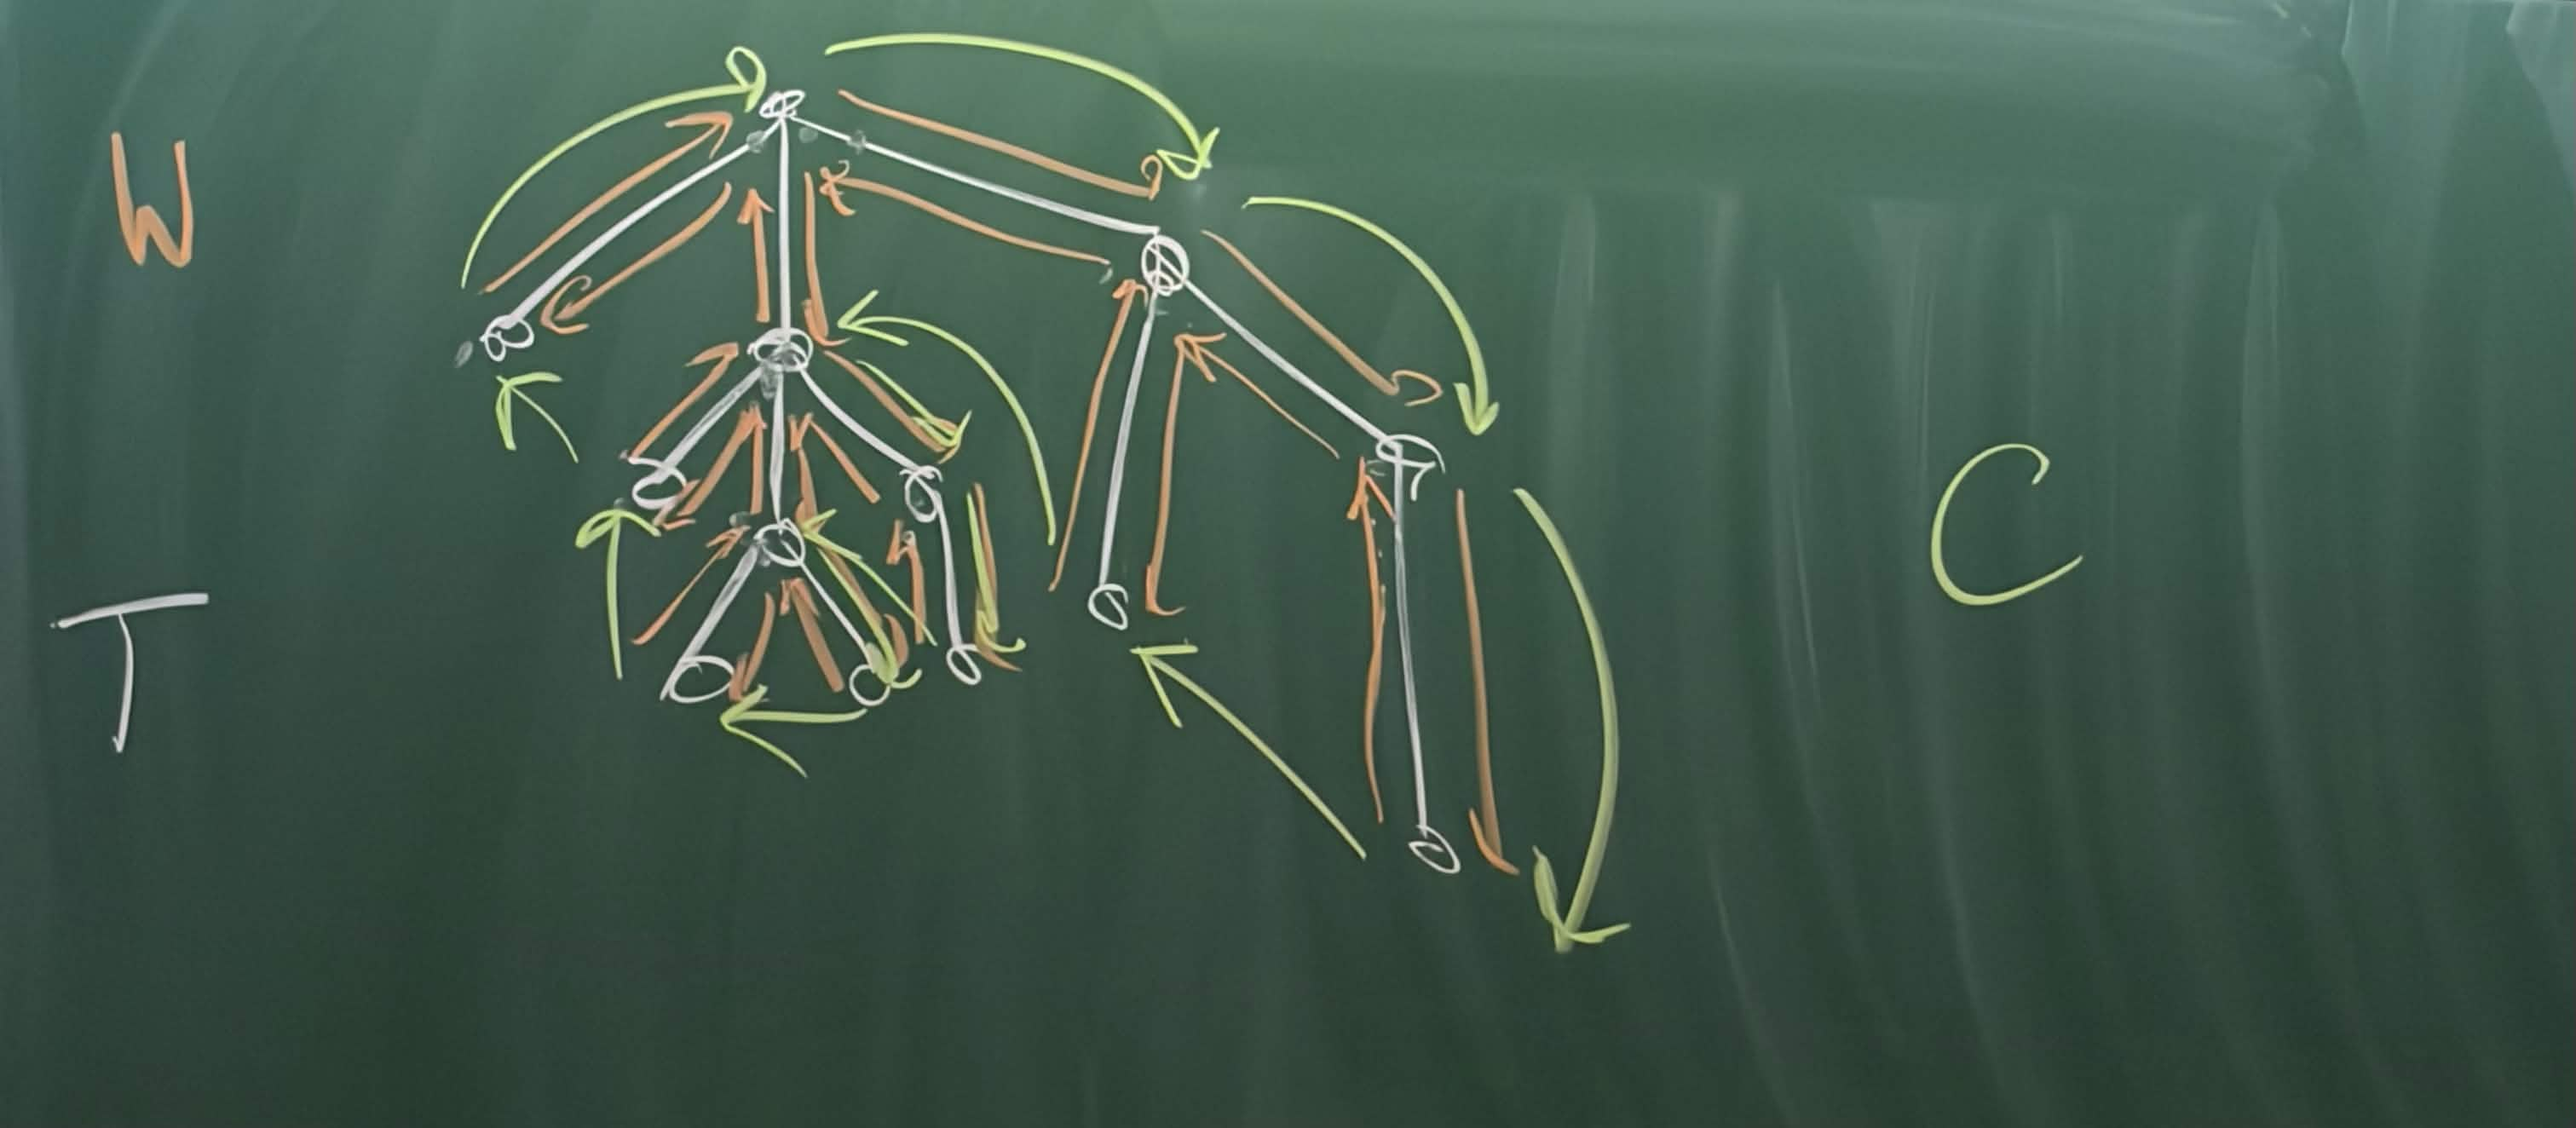
\includegraphics[width=0.8\textwidth]{./Figures/2approximation.jpg}
    \end{figure}
    Hence,
    \[
        w(C) \le 2 w(C^*).
    \]
\end{proof}

\section{Maximum matching}
\begin{question}
    How do we find a maximum matching?
\end{question}

\begin{remark}
    Maximum is not equal to maximal, where maximum means largest there is, and maximal means cannot be extended.
\end{remark}

\begin{claim}
There exists a simple \( \tfrac{1}{2} \)-approximation algorithm for the maximum matching problem.
\end{claim}

\begin{explanation}
Consider the following greedy algorithm: process the edges of \( G \) in an arbitrary order, and add an edge to the matching \( M \) if it is disjoint from all previously selected edges. The resulting matching \( M \) is \emph{maximal}.

Let \( M^* \) be a maximum matching. We claim that
\[
|M^*| \le 2|M|.
\]

Since \( M \) is maximal, no edge in \( E(G) \setminus M \) can be added to \( M \). In particular, for every edge \( e = (u,v) \in M^* \), at least one of its endpoints must already be saturated by \( M \); otherwise, \( e \) could be added to \( M \), contradicting maximality.

Thus, for every edge \( e \in M^* \), we can choose one endpoint that is saturated by \( M \). Define a mapping
\[
f : M^* \to V(M)
\]
by assigning each edge \( e \in M^* \) to one of its endpoints that is saturated by \( M \).

We now show that \( f \) is injective. Suppose \( e_1, e_2 \in M^* \) are distinct edges such that
\[
f(e_1) = f(e_2) = v.
\]
Then both \( e_1 \) and \( e_2 \) are incident to \( v \), which contradicts the fact that \( M^* \) is a matching. Hence, \( f \) is injective.

Therefore,
\[
|M^*| \le |V(M)|.
\]
Since every edge in \( M \) saturates exactly two vertices and no two edges share a vertex,
\[
|V(M)| = 2|M|.
\]
Combining the inequalities, we obtain
\[
|M^*| \le 2|M| \quad \Longrightarrow \quad |M| \ge \tfrac{1}{2}|M^*|.
\]

Thus, the greedy algorithm produces a \( \tfrac{1}{2} \)-approximation.
\end{explanation}

\begin{definition}
    Let \(G\) be a graph and let \(M \subseteq E(G)\) be a matching. An \(M\)-alternating path is a path where every alter edge is in \(M\). An \(M\)-augmenting path is an \(M\)-alternating path whose endpoints are unsaturated by \(M\).       
\end{definition}

\begin{theorem}[Berge, 1953]
Let \( G \) be a graph and let \( M \subseteq E(G) \) be a matching. Then \( M \) is a maximum matching if and only if there is no \( M \)-augmenting path.
\end{theorem}

\begin{proof}
\hfill

\paragraph{(\(\implies\))} 
Suppose that \( M \) is a maximum matching. We show that there is no \( M \)-augmenting path.

Assume for contradiction that there exists an \( M \)-augmenting path \( P \). By definition, \( P \) is an alternating path whose edges alternate between edges not in \( M \) and edges in \( M \), and whose endpoints are \emph{unsaturated} by \( M \) (i.e., not incident to any edge in \( M \)).

Define
\[
M' := M \,\Delta\, E(P).
\]
Since \( P \) is alternating, this operation replaces the edges of \( M \) on \( P \) with the edges not in \( M \). Because both endpoints of \( P \) are unsaturated by \( M \), the path contains one more edge not in \( M \) than in \( M \). Hence,
\[
|M'| = |M| + 1.
\]

\begin{center}
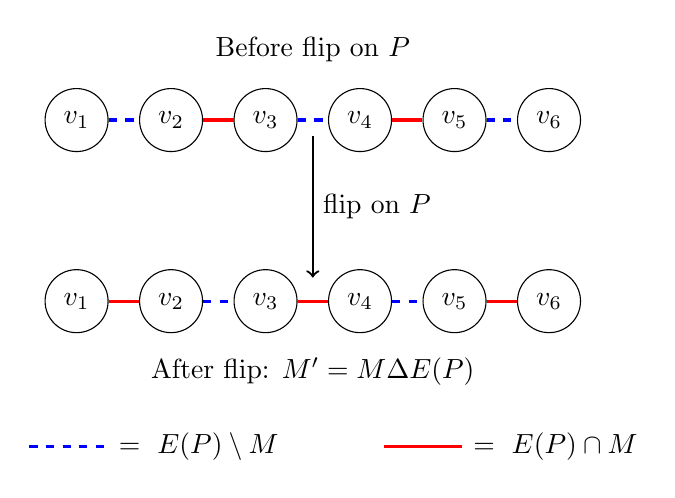
\begin{tikzpicture}[
  v/.style={circle, draw, fill=white, minimum size=8mm, inner sep=1pt},
  medge/.style={line width=1.2pt},
  augedge/.style={line width=1.2pt, dashed}
]
  % Before flip
  \node[v] (t1) at (0,0) {$v_1$};
  \node[v] (t2) at (1.2,0) {$v_2$};
  \node[v] (t3) at (2.4,0) {$v_3$};
  \node[v] (t4) at (3.6,0) {$v_4$};
  \node[v] (t5) at (4.8,0) {$v_5$};
  \node[v] (t6) at (6.0,0) {$v_6$};

  \draw[augedge, blue] (t1)--(t2);
  \draw[medge, red] (t2)--(t3);
  \draw[augedge, blue] (t3)--(t4);
  \draw[medge, red] (t4)--(t5);
  \draw[augedge, blue] (t5)--(t6);
  \node at (3.0,0.9) {Before flip on $P$};

  % After flip
  \node[v] (b1) at (0,-2.3) {$v_1$};
  \node[v] (b2) at (1.2,-2.3) {$v_2$};
  \node[v] (b3) at (2.4,-2.3) {$v_3$};
  \node[v] (b4) at (3.6,-2.3) {$v_4$};
  \node[v] (b5) at (4.8,-2.3) {$v_5$};
  \node[v] (b6) at (6.0,-2.3) {$v_6$};

  \draw[medge, red] (b1)--(b2);
  \draw[augedge, blue] (b2)--(b3);
  \draw[medge, red] (b3)--(b4);
  \draw[augedge, blue] (b4)--(b5);
  \draw[medge, red] (b5)--(b6);
  \node at (3.0,-3.2) {After flip: $M' = M \Delta E(P)$};

  % Arrow from before to after (centered)
  \draw[->, thick] (3.0,-0.2) -- (3.0,-2.0) node[midway, right] {flip on $P$};

  % Centered legend (symmetric)
  \draw[augedge, blue] (-0.6,-4.15) -- ++(1.0,0)
    node[right, black] {$=\ E(P)\setminus M$};
  \draw[medge, red] (3.9,-4.15) -- ++(1.0,0)
    node[right, black] {$=\ E(P)\cap M$};
\end{tikzpicture}
\end{center}

Moreover, \( M' \) is still a matching, since along the path we never create two edges sharing a common endpoint.

This contradicts the maximality of \( M \). Therefore, no \( M \)-augmenting path exists.

\paragraph{(\(\impliedby\))} 
Suppose that there is no \( M \)-augmenting path. We show that \( M \) is a maximum matching.

Let \( M^* \) be a maximum matching in \( G \), and consider
\[
H := M \,\Delta\, M^*.
\]
Each vertex in \( H \) has degree at most 2, since both \( M \) and \( M^* \) are matchings. Thus every connected component of \( H \) is either an even cycle or a path. Moreover, each component is alternating between edges in \( M \) and edges in \( M^* \).

Consider a path component \( P \). Along \( P \), the edges alternate between \( M \) and \( M^* \), so the numbers of edges from the two matchings differ by at most one.

If \( |M^*| > |M| \), then there must exist a component \( P \) in which the number of edges from \( M^* \) exceeds the number from \( M \). Such a component must be a path whose first and last edges lie in \( M^* \).

Therefore, the endpoints of \( P \) are not incident to any edge in \( M \), i.e., they are \emph{unsaturated} by \( M \). Hence, \( P \) is an \( M \)-augmenting path.

\begin{center}
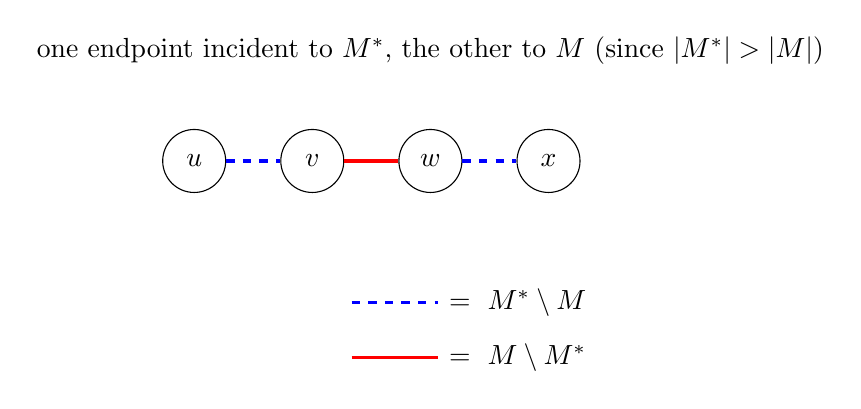
\begin{tikzpicture}[
  v/.style={circle, draw, fill=white, minimum size=8mm, inner sep=1pt},
  medge/.style={line width=1.2pt, red},
  mstar/.style={line width=1.2pt, blue, dashed}
]

  % Case 2: one endpoint M*, other M (difference still not +1 for M*)
  \node at (3,-2.0) {one endpoint incident to $M^*$, the other to $M$ (since \(\vert M^* \vert > \vert M \vert \))};
  \node[v] (a2) at (0,-3.4) {$u$};
  \node[v] (b2) at (1.5,-3.4) {$v$};
  \node[v] (c2) at (3.0,-3.4) {$w$};
  \node[v] (d2) at (4.5,-3.4) {$x$};
  \draw[mstar] (a2)--(b2);
  \draw[medge] (b2)--(c2);
  \draw[mstar] (c2)--(d2);

  % Centered legend using line segments (stacked to avoid overlap)
  \draw[mstar] (2.0,-5.2) -- ++(1.1,0) node[right, black] {$=\ M^*\setminus M$};
  \draw[medge] (2.0,-5.9) -- ++(1.1,0) node[right, black] {$=\ M\setminus M^*$};
\end{tikzpicture}
\end{center}

This contradicts the assumption that no such path exists. Therefore, \( |M| = |M^*| \), and thus \( M \) is a maximum matching.
\end{proof}